This section describes commercially available real-time oscilloscopes, as well as the \gls{kapture} system, which is in use at \gls{kara} for \gls{thz} diagnostics. Understanding the architecture of the latter will help for the development of the new system, as the basic concept of \gls{kapture} is reused there.
\section{Real-Time Oscilloscope}
\begin{itemize}
	\item KeySight Infiniium MXR-Series Real-Time Oscilloscopes
	\item Rohde\&Schwarz DPO70000SX
	\item LeCroy LabMaster 10-100Zi
\end{itemize}

\section{\gls{kapture}}
\Gls{kapture} is a fast readout system developed at the \Gls{ipe} for \Gls{thz} diagnostics at \gls{kara}. It is designed to digitize the pulses generated by \Gls{thz} detectors at each revolution, only sampling the pulse shapes without the "empty" signal in between. The system is able to sample pulses with a \gls{fwhm} between a few tens to a hundred picoseconds with a minimal sample time of \SI{3}{\pico \second}. \cite{caselleKAP}

\subsection{General Architecture}
The system consists of two parts: the sampling front-end card and a \gls{fpga} readout card. In \autoref{fig:thz_chain} the setup for \gls{thz} radiation measurements with \gls{kapture} is shown. 

The incoming radiation is fed into a detector, which converts the incident photons into an electrical signal. This signal is then amplified in a wide-band \gls{lna}. The latter splits the detector signal into four identical signals, which are then propagated to the sampling front-end card. The card consists of four parallel sampling channels with adjustable sample time, each containing a \gls{tha} and an ADC. This card is connected to a read-out card, which has two tasks: programming the components on the front-end card (\gls{fpga}-part) and sending the acquired data to a PC/\gls{daq} system. \cite{caselle2014}

\begin{figure}[tbh]
	\centering
	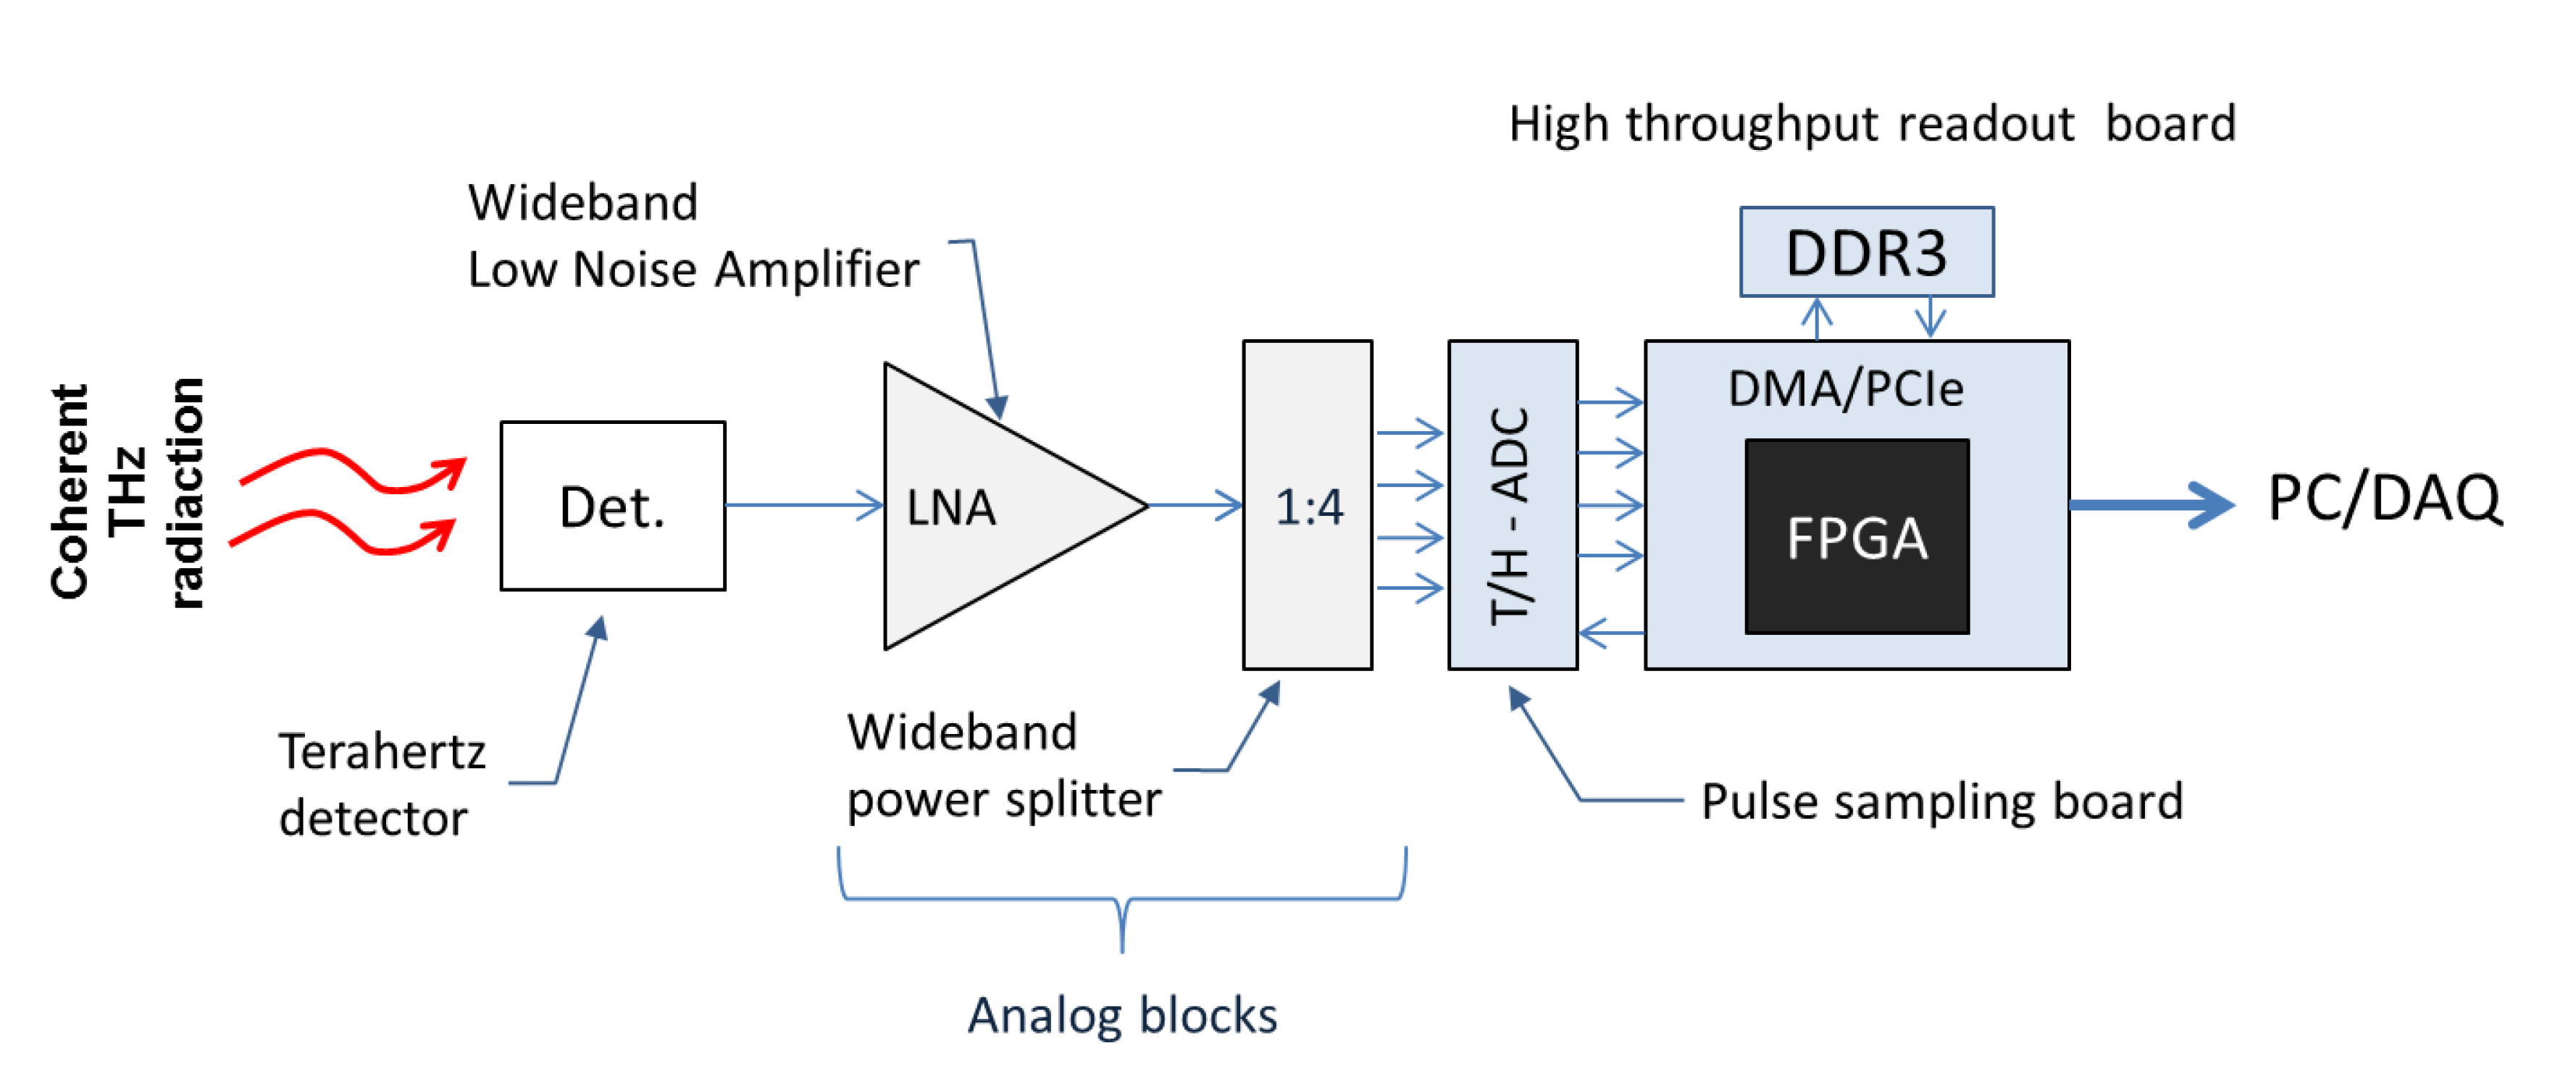
\includegraphics[width = \textwidth]{chap/03-currentStat/img/thz_chain}
	\caption[THz measurement with KAPTURE]{\gls{thz} radiation measurement setup with \gls{kapture}(cf. \cite{caselle2014})}
	\label{fig:thz_chain}
\end{figure}

\subsection{Analog front-end}
Due to the high bandwidth nature of the detector signal, the analog front-end of the system has to be wideband as well to be able to sample the signal with picosecond resolution. 

The used \gls{lna} is based on a commercial GaAs \gls{mmic} which operates from DC to \SI{50}{\giga \hertz}. It is needed to compensate the insertion loss\footnote{\textit{Insertion loss} is the loss of signal power which occurs, when a signal passes through a component.} due to the following power splitter. %todo maybe more info, ask michele

Classical power-splitters are not intrinsically wideband (\cite{caselle2014}). For that reason, an wideband power-splitter was developed at \gls{ipe} which fulfills the bandwidth requirements. The designed power-splitter works up to \SI{100}{\giga \hertz} with an insertion loss of \SI{8}{\decibel} and a return loss\footnote{\textit{Return loss} is the loss of signal power due to reflection by a discontinuity in the transmission line.} of about \SI{20}{\decibel} at \SI{50}{\giga \hertz}.\cite{caselle2014}

\subsection{Sampling board}
The general structure of the board with the power splitter is shown in \autoref{fig:kapture}. 
\begin{figure}[tbh]
	\centering
	\includegraphics[width = \textwidth]{chap/03-currentStat/img/kapture.tikz}
	\caption{General architecture of the KAPTURE front-end sampling card (cf. \cite[p.2]{caselleKAP})}
	\label{fig:kapture}
\end{figure}

Four identical signals from the power-splitter are fed into four channels, consisting of a respective \gls{tha} unit and a 12-bit \gls{adc} sampling at \SI{500}{\mega\sample\per\second}. The sampling time of each unit can be adjusted individually with a delay chip with a resolution of \SI{3}{\pico \second} (maximal delay range: \SI{100}{\pico \second}). The delay chips are programmed with the \gls{fpga} on the readout card.
The clock signal is provided by \gls{kara}, which is cleared from jitter by a \gls{pll}. This ensures the synchronization of the \glspl{adc} with the \gls{rf} system. The cleaned clock signal is distributed to the delay chips via fan-out buffer. \cite{caselleKAP}
In this way, the pulse can be "locally sampled" by adjusting the different delay with a maximum rate of 330 GS/s possible. 
A simplified representation of the local sampling of the signal is shown in \autoref{fig:detector_signal}.
\begin{figure}[tbh]
	\centering
	\includegraphics[width = \textwidth, height=0.4\textwidth]{chap/03-currentStat/img/detector_signal.tikz}
	\caption{Signal and sampled points $S_1$ to $S_4$}
	\label{fig:detector_signal}
\end{figure}

\autoref{fig:kapturesys} shows a photo of the system setup at \gls{kara}
\begin{figure}[tbh]
	\centering
	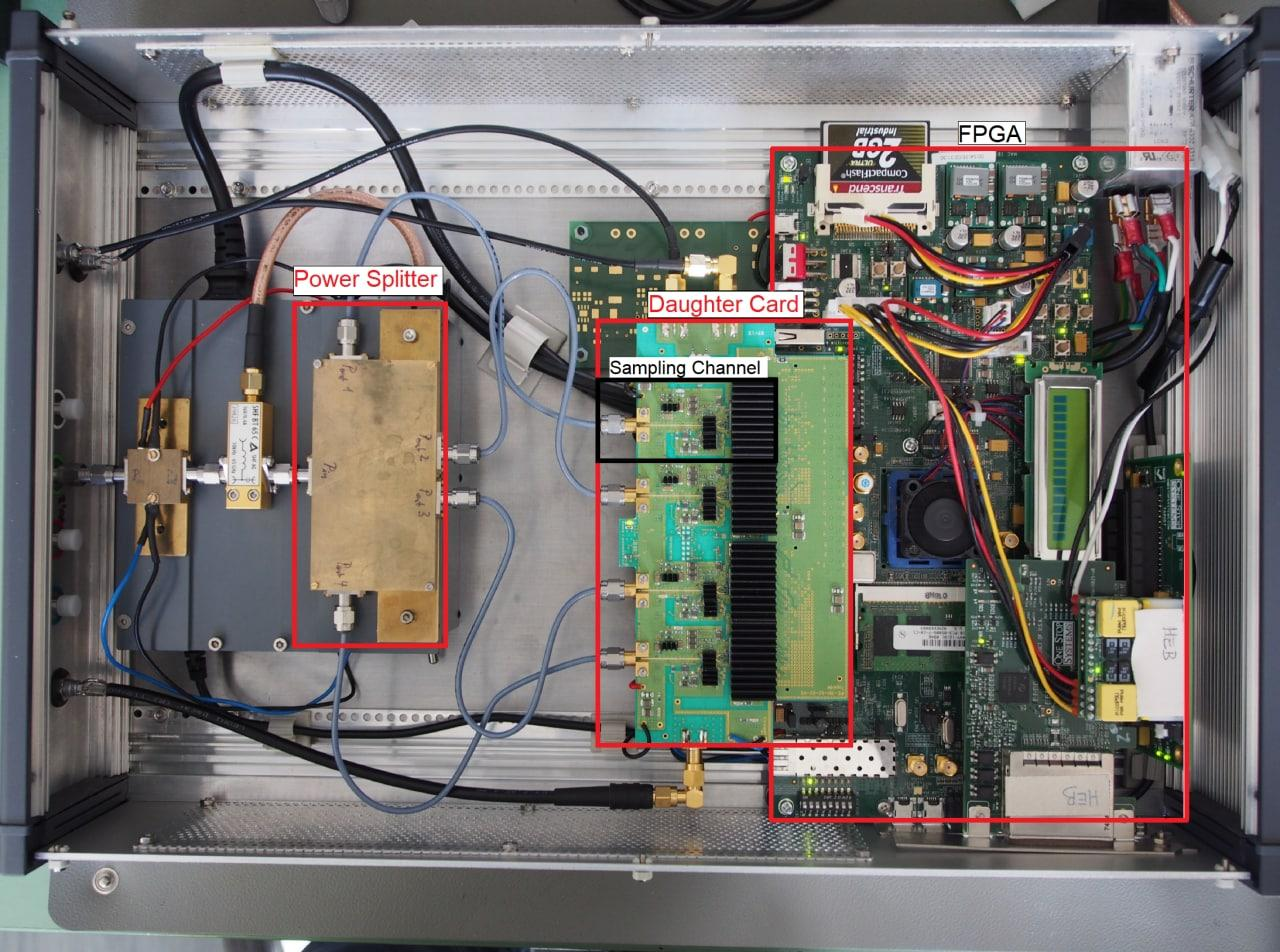
\includegraphics[width = \textwidth]{chap/03-currentStat/img/kapture_sys}
	\caption{Photo of KAPTURE with highlighted main components. \cite[p.~61]{brosi}}
	\label{fig:kapturesys}
\end{figure}
%todo  re-label

\subsection{FPGA-GPU architecture}

In order to keep a continuous data acquisition the necessary bandwidth is 
\begin{equation}
	12 \text{bits} \cdot 4 \, \text{samples} \cdot \SI{500}{\mega \hertz} = 24 \text{Gb/s}
\end{equation}
To ensure high data throughput, the readout board is based on a bus master DMA architecture which is connected to \gls{pcie} end-point logic. This ensure a throughput of up to 2 GByte/s. \cite{caselleKAP}

\subsection{KAPTURE-2}

\begin{figure}[tbh]
	\centering
	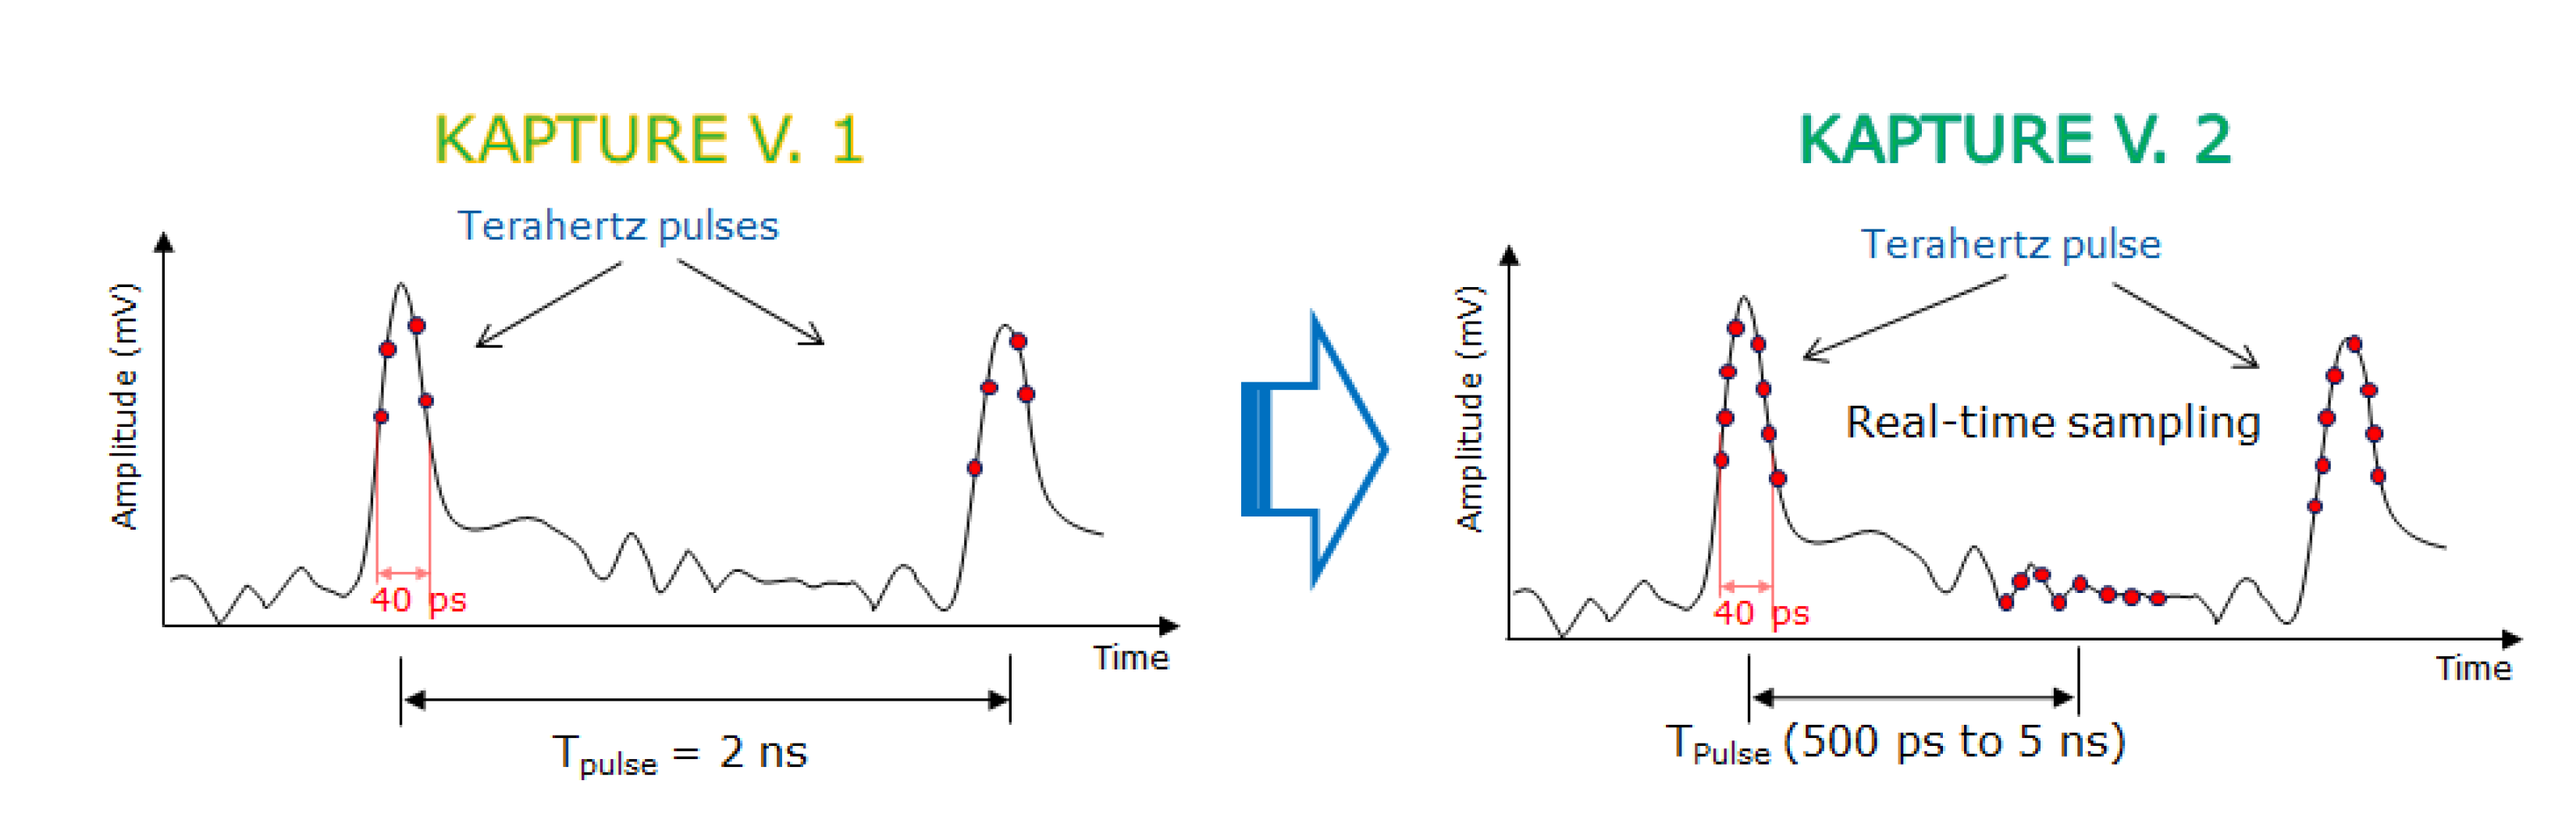
\includegraphics[width = \textwidth]{chap/03-currentStat/img/kap1_vs_kap2}
	\caption{Comparison between KAPTURE and KAPTURE-2\cite{caselleKAP}}
	\label{fig:kap1vskap2}
\end{figure}
